\documentclass[authoryear,review,11pt]{elsarticle}
\bibliographystyle{elsarticle-harv}
\usepackage{graphicx}
\usepackage{amsmath, amsfonts, amssymb, latexsym, inputenc, moreverb, wrapfig, subfigure, array, setspace, cite}
\usepackage{lineno}
\linenumbers
\usepackage{subfigure}
\usepackage[pdftex]{color}
\definecolor{darkblue}{rgb}{0,0,0.5}
\definecolor{darkgreen}{rgb}{0,0.5,0}
%\usepackage[pdftex, colorlinks, citecolor=darkblue,linkcolor=darkgreen]{hyperref}
\usepackage[pdftex, colorlinks]{hyperref}
\textwidth 6.75in
\oddsidemargin -0.15in
\evensidemargin -0.15in
\textheight 9in
\topmargin -0.5in
\newcommand{\ud}{\mathrm{d}}
\newcommand{\degree}{$^{\circ}$}
\newcommand{\tb}[1]{\textcolor{blue}{#1}} 
\newcommand{\E}{\text{E}}



 
\begin{document}
\begin{frontmatter}
\title{Where Is All the Sympatric Speciation?  \\ Stochastic Impediments to Evolutionary Branching}
\author[carl]{Carl Boettiger\corref{cor1}}
\ead{cboettig@ucdavis.edu}
\cortext[cor1]{Corresponding author.}
\author[rupert]{Rupert Mazzucco\corref{cor1}}
\ead{mazzucco@iiasa.ac.at}
\author[ulf]{Ulf Dieckmann\corref{cor1}}
\ead{dieckmann@iiasa.ac.at}
\address[carl]{Center for Population Biology, University of California, Davis, United States}
\address[rupert]{International Institute for Applied Systems Analysis, Austria}
\address[ulf]{International Institute for Applied Systems Analysis, Austria}
\begin{abstract}
While empirical evidence leans almost entirely in favor of allopatric speciation, theoretical evolutionary models continue to suggest that sympatric speciation should be possible, even common.  We show stochastic effects due to finite population sizes can pose a significant impediment to the evolutionary branching.  Early in branching, coexistence of the diverging populations is protected by a very weak stabilizing force, as trait differences are still small.  Consequently stochastic collapse of this weak coexistence is common on the evolutionary timescale required for mutation-limited divergence.  Sympatric branching mechanisms require an evolutionary divergence to occur fast enough to prevent this eventual collapse.  Either rapid mutations or mutations of large effect are required to traverse this branching point successfully – or otherwise a population that begins to diverge in allopatry can find its branching reinforced upon second contact by these sympatric effects.  
\end{abstract}
\begin{keyword}
Evolution \sep demographic stochasticity \sep branching \sep adaptive dynamics
\end{keyword}
\end{frontmatter}
\section{Introduction}
Speciation is evolution at the grandest scale. Speciation is the mechanism responsible for generating the astounding biodiversity that is the most salient feature of life on Earth, and one of our most threatened and irreplaceable resources. Speciation is also one of the greatest mysteries of evolution, occurring primarily on scales of space and time beyond our experimental reach, and through a delicate interplay of events from the molecular shifting of nucleotides to the geologic shifting of mountains and rivers. For organisms with sexual reproduction, the process of speciation must account for the genetic isolation of incipient species, and speciation models must therefore embrace genetic dynamics (Coyne \& Orr 2004). Accounting for this genetic dimension of speciation has been achieved largely at the expense of simplifying, or ignoring altogether, speciation’s ecological dimension. The latter results from the complex features and interactions that distinguish species from one another and that enable a rich diversity of species to persist.

The importance of ecological interactions in speciation has been acknowledged for some time (the concept of reinforcement goes back to Dobzhansky and Wallace), yet few studies have had more influence in highlighting the ecological basis for speciation then that by Dieckmann and Doebeli (1999), which brought the nascent theory of mutation-limited long-term phenotypic evolution known as ‘adaptive dynamics’ to the attention of empirical and theoretical evolutionary ecologists. While genetic dynamics are addressed in this study, at its heart lies an ecological model for the evolutionary branching of a phenotypic trait describing competitive interactions: in the course of adaptation, this trait approaches an evolutionary branching point, i.e., an attractor of the evolutionary dynamics of a single morph that, once reached through directional selection, naturally leads to the emergence of a diverging dimorphism through frequency-dependent disruptive selection. In this project, we will focus on the dynamics around such evolutionary branching points. While ignoring genetic details for a start, we will extend previous work by focusing on the impacts of stochastic processes on the evolutionary dynamics leading to biological diversification.

Almost all quantitative theories of evolution have relied on stochastic models to address the impacts of chance events – such as mutations, births, deaths, and environmental changes – that affect the evolutionary process (Fisher 1937; Lande 1979; Coyne \& Orr 2004). Adaptive dynamics theory typically considers two sources of stochasticity: random mutations and the loss of advantageous mutants to chance extinction while their numbers are small. What these models typically do not consider is demographic stochasticity of resident populations (resulting from intrinsic fluctuations through stochastic birth and death events in finite populations of discrete individuals) and environmental stochasticity (resulting from external fluctuations in the environmental conditions a population experiences).


Several recent studies have tried to overcome these limitations. Claessen et al. (2007, 2008) explore simulations of evolutionary branching in small populations and found that demographic stochasticity can delay or halt diversification. Johansson and Ripa (2006) explored the impact that correlated  environmental stochasticity has on diversification. They assume that as populations diverge, the environmental influences upon them become less similar. They demonstrate that this correlation can facilitate coexistence early in the process of branching, and as it weakens, the chance that a branch is lost increases. While these studies make an excellent start, a more general theory and mathematical framework is needed to untangle and quantify the multitude of effects stochasticity has on evolutionary branching.


\section{Methods}
\subsection{Model}
We consider the classic adaptive dynamics model for evolutionary branching under competition for a limiting resource by Dieckmann and Doebeli (1999).  The population dynamics of $N(x,t)$ individuals each with focal trait $x$ are given by a continuous time birth-death process with rates 
\begin{align}
b(N) = & r \nonumber \\
d(N) = & r \frac{\sum_yN(y,t)C(x,y)}{K(x)} .\label{general_logistic}
\end{align}
The focal trait $x$ can be thought of as some continuous phenotypic variable, such as beak size, which affects resource consumption.  Niche differences driving speciation arise from differences in this trait.  In the model, $K(x)$ is the resource kernel which determines the equilibrium population density and $C(x,y)$ is a the competition kernel, describing the relative change in death rate of individuals of type $x$ due to competition by individuals of type $y$.  Given $C(x,x)=1$, the equilibrium density of a monomorphic population is $N^{\ast}(x)=K(x)$.  Following~\citet{dieckmann_nat1999} we assume the following Gaussian forms,
\begin{equation}
K(x)=K_0e^{-x^2/(2\sigma_k^2)}, \label{K}
\end{equation}
and
\begin{equation}
C(x,y)=e^{-(x-y)^2/(2\sigma_c^2)}, \label{C}
\end{equation}
where $\sigma_k$ and $\sigma_c$ are scale factors for the resource distribution and competition kernels respectively.  $\sigma_c$ can be though of as the niche size.  We focus on the case $\sigma_k>\sigma_c$, for which the model has an evolutionary branching point at $x=0$~\citep{geritz_evoeco1998}.  

The evolutionary dynamics are specified only at the phenotypic level: We assume that with probability $\mu$ an individual birth results in a mutant offspring, and that the mutant trait is chosen from a Gaussian distribution centered at the trait value of the parents and with a variance $\sigma_{\mu}^2$. 


\subsection{The Adaptive Dynamics of Branching}
%% pip with coexistence region, P_2, sample trajectory in PIP

\begin{figure}[h]
\begin{center}
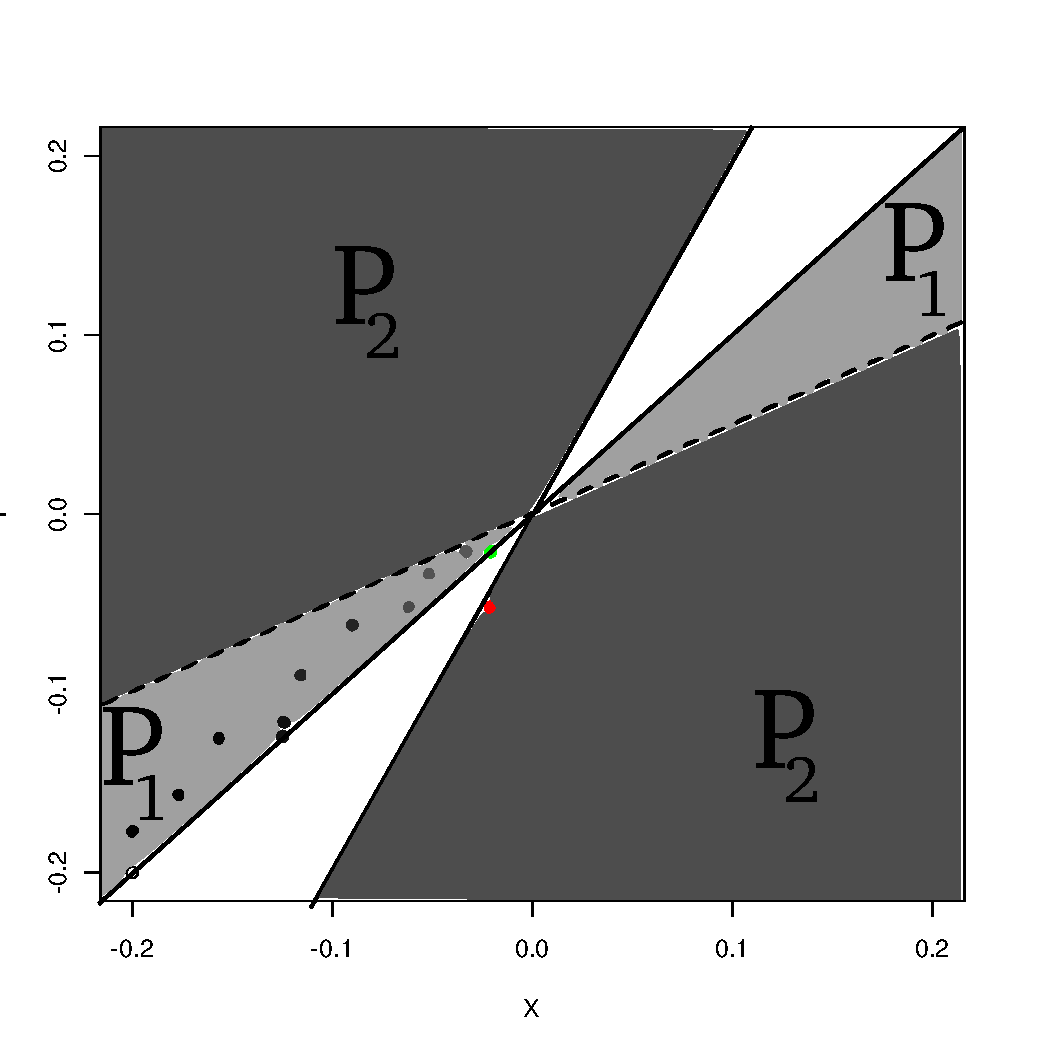
\includegraphics[width=\textwidth]{jump_void2.pdf}
\end{center}
\caption{\textbf{Jumping the void}. Pairwise invasibility plot showing a sample trait substitution sequence that eventually enters the coexistence region, $P_2$.  Positive fitness regions of the plot are shaded.  The lighter shaded region, denoted $P_1$, corresponds to mutants that are expected to successfully invade and replace the resident.  The darker shading $P_2$ corresponds to mutants expected to successfully invade but coexist with the resident population.   Dots indicate a sample run of the the evolutionary process -- showing which mutant values (on the Y axis) successfully invade their resident populations (on the x axis).  The sequence approaches the branching point, finally jumping into the coexistence region at the trait value colored in red.  }
\label{fig:pip}
\end{figure}

Evolutionary branching occurs in this model when the resource kernel is wider than the competition kernel, $\sigma_k > \sigma_c$ as discussed in~\citet{geritz_evoeco1998, dieckmann_nat1999}.  It is straight forward to show that the invasion fitness $s(y,x) := b(K(x),x,y) -d(K(x), x,y)$ of a rare mutant $y$ in a population $x$ at equilibrium has a singular point at $x^*=0$, the peak of the resource distribution.  This is easily confirmed by taking the second derivatives or observing the pairwise invasibility plot~\ref{fig:pip}.  


\subsection{Phases of branching}
Evolutionary branching through this mechanism can be divided into four phases.  In the first phase, the population approaches the branching point by repeated invasions that completely replace the monomorphic population.  This rate is governed by the canonical equation of adaptive dynamics, a rate proportional to the size of mutational jumps relative to the size of the resource kernel, $\sigma_{\mu}/\sigma_k$.  Mathematically, this phase can be defined by the $P_1$ region of the pairwise invasibility plot.  In this region, dimoprhisms are always transient.  

In the second phase, the population is near enough to the branching point that mutations begin occuring in the coexistence region.  More precisely, any dimorphism that occurs in the $P_2$ region but where one of the populations is too small to contribute to density-dependent effects can be considered to be in this phase.  The dynamics of this phase are thus governed by the fixation probabilities of rare mutants occuring in the coexistence region.  This phase may often fail when a rare mutant occurs in the coexistence region but is soon lost to drift.  

The third phase begins when mutations in the coexistence region survive the initial genetic drift to establish as significant frequencies in the population.  In this stage the density-dependent contribution of each population is relevant.  This stage may fail due to the loss of either population, more often the one farther from the branching point.  As this is usually (but not necessarily) the resident population that gave rise to the other population through mutation, the failure of this phase can be thought of in terms of loss of the resident population, while the second phase is governed primarily by the loss of the invader population.  

In the fourth phase, subsequent mutations farther from the branching point invade and the populations move apart.  Each time a mutant exterior to the branching point successfully invades the probability the coexistence becomes exponentially more stable, as we will demonstrate.  While the expected coexistence time for the two populations remains similar to the evolutionary timescale over which new mutants enter and establish, the coexistence may be lost, collapsing back to the second phase.  However, as the coexistence of the first pair (phase 3) is much more likely to collapse than the subsequently more stable coexisting pairs that arise from it, we will have a good approximation by considering only the probabilty that the initial pair survives long enough to enter phase four.  This is justified by the Ahrennius approximation result and confirmed by numerical simulation.


\subsubsection{Overview of the approach}
The division into phases provides both a conceptual and mathematical framework to address the branching process.  Analyzing the first two phases essentially consists of partitioning the space of possible mutants: considering all the mutants that lie in the $P_1$ region that are expected to invade and replace the resident (moving the population closer to the branching point as per phase 1), and mutants that reach the coexistence region $P_2$ in phase 2.  This is done by partitioning the domain of integration for an integral over mutant traits $y$ for each resident $x$.  The closer $x$ is to $x^*$ the more of this integral lies in $P_2$ and entering phase two becomes increasingly probable.  This treatment follows along similar lines as the original derivation of the canonical equation of adaptive dynamics~\citep{dieckmann_jmb1996}.  

The crux of the remaining third and fourth phases settles around predicting the coexistence time.  This is done through a diffusion approximation approach to individual dynamics, which remains quite technical to solve.  To provide both an effective approximation and a useful intuition, we demonstrate how this coexistence problem can be construed as an escape from a potential energy well, as in classical chemical kinetics.  Understanding the depth of this well tells us most of what we need to know about the coexistence time.  Relating the coexistence timescale to the evolutionary timescale wraps up the calculation for how long branching will take.  

The deterministic theory applies both the limit of rare mutations (small $\mu$) and small mutational steps (small $\sigma_{\mu}$).  In our treatment, either one of these can become the limiting factor and correspond to different regimes of adaptive branching.  If mutations are very rare, we'll see that the population must essentially survive phase 3 in a single mutational step.  In this regime recieving a single mutation far enough into the $P_2$ region to survive the coexistence balance (phase 3 to 4).  This corresponds to a single mutational step that is on the order of the width of the competition kernel, $\sigma_c$.  Here branching is accomplished essentially by the single unlikely event being ``rolled,'' and transitions between phases are slow but rarely collapse to an earlier stage.  When mutational step size is limiting, many mutational steps are required to get any population a distance of order $\sigma_c$ away -- to escape the shadow of competition.  In this regime, successful branching appears as a lucky string of mutations, like a long series of flipping a coin and coming up heads rather than the singular improbable event.  This regime is characterized by many aborted branching attempts before one succeeds.  The smaller $\mu$ becomes, the smaller the chances of seeing this lucky run within the coexistence time.  The smaller $\sigma_{\mu}$ becomes the smaller the chances of seing the rare large jump within the coexistence time.  When both are too small relative to the coexistence time, the population will fail to branch.  


\subsection{Approaching the branching point}
Classically, the approach to the branching point is governed by the canonical equation of adaptive dynamics~\citep{dieckmann_jmb1996}.  To account for branching we have to revisit the original derivation of this equation where we relax the limit of small mutational steps sufficiently to allow mutants to enter the coexitence region, $P_2$, in Fig.~\ref{fig:pip}.  The derivation of the canonical equation integrates only over those mutants that fall into the invasion-substitution region, $P_1$.  However, since the derivation is done in the limit of small mutational step sizes, this encompasses essentially all of the weight of the mutational kernel, and to good approximation can thus be replaced with the entire $P_1 \cup P_2$ region.  Recall that in the derivation of the canonical equation, deleterious mutations are given zero probability of fixing (from the branching process approximation), and hence this corresponds to integrating over half of the real line $\mathbb{R}$.  

\begin{align}
\frac{\ud \bar x}{\ud t} = \mu N^*(x) \phantom \cdot \partial_y s(y,x) \Big|_x \int_{P_1} [y-x]^2 M(y-x) \ud [y-x]
\label{canonical}
\end{align}

The probability of such a mutant occurring in our monomorphic population of trait $x$ is given by the probability that any mutant occurs (given by the population size, approximately $K(x)$ at equilibrium, times the birth rate $b(x)$ times the mutation rate $\mu$) times the probability that the mutation lies on the opposite side of the coexistence boundary, which we denote as $\phi(x)$ and $\psi(x)$, which is $\phi(x)$ reflected across the line $y=x$.  This depends on the mutational kernel, $M(y,x)$ which gives the probability that a mutant arising from a resident population of trait $x$ bears trait $y$ that falls withing the coexistance region as follows:

\begin{equation*}
\int_{-\infty}^{\phi(x)} M(y,x) \ud y + \int_{\psi(x)}^{\infty} M(y,x) \ud y 
\end{equation*}
Without loss of generality let us assume that the singular strategy $x^* = 0$ and that we start from some trait value $x_0 > x^*$.  Additionally, let us we assume $M(y,x)$ is Gaussian in $y-x$ with mean 0 and variance $\sigma_{\mu}^2$. However, we do not wish to consider all such mutants $y$, but only those that survive.  We multiply the probability of a mutant having trait $y$, $M(y,x)$, times the probability that is survives drift.  This probability we quote from the Galton-Watson branching process, $1-\tfrac{d(y,x)}{b(y,x)}$. Using our model for birth and death rates~\eqref{general_logistic}, the probability of surviving branching is

\begin{equation}
1-\frac{C(y,x)K(x)}{K(y)} := S(y,x)
\label{S}
\end{equation}

which we denote as $S(y,x)$ as indicated. Hence we modify our integral to consider all mutants $y < x^*$ which occur with probability $M(y,x)$ and then survive with probability $S(y,x)$, and write down the rate $P(x)$ at which a mutant which leads to branching occurs from our monomorphic population with trait $x$:

\begin{equation}
P(x) := r \mu K(x)\left( \int_{-\infty}^{\phi(x)} M(y,x) S(y,x) \ud y + \int_{\psi(x)}^{\infty} M(y,x) S(y,x) \ud y  \right)
\label{MSerf}
\end{equation}

Though a little cumbersome, this can be written in nearly closed form (using the error function). For our particular model $s(y,x)$, we can write the boundaries $\phi(x)$ and $\psi(x)$ as 

\begin{align}
\phi(x) = x\frac{\frac{\sigma_k^2}{\sigma_c^2}+1}{\frac{\sigma_k^2}{\sigma_c^2}-1} \nonumber \\
\psi(x) = x\frac{\frac{\sigma_k^2}{\sigma_c^2}-1}{\frac{\sigma_k^2}{\sigma_c^2}+1}
\label{phipsi}
\end{align}
Then, given a starting condition $x_0$, we can determine the expected trait $x$ at time $t$ of a monomorphic resident population by integrating the canonical equation,

\begin{equation}
\frac{\ud x}{\ud t} = \frac{1}{2} \mu \sigma_{mu}^2 N^*(x) \partial_y s(y,x)
\end{equation}

which for our model is  
\begin{equation}
\frac{\ud x}{\ud t} = \frac{-x}{2\sigma_k^2} r \mu \sigma_{\mu}^2 K(x) 
\end{equation}
While no closed form solution exists for $x(t)$ in this case, if we assume $x_0 \ll \sigma_k$ then to good approximation we can view $K(x)$ to be constant over the interval and take our path to be:

\begin{equation}
x(t) = x_0 \exp\left( -r \mu \sigma_{\mu}^2 K_0 t/\sigma_k^2\right)
\end{equation}

Using this mean path, we can write down an approximation for the rate of a branching mutant occurring as a function of time, $P(x(t))$.  Using this time dependent rate, the probability of not branching after time $T$ is simply $\exp\left( - \int_0^T P(t)\ud t \right)$.  One minus this is the probability branching by time $T$; i.e. the cumulative density function, hence the probability density function for the waiting time is:

\begin{equation}
\Pi(T) = P(x(T)) \exp\left( -\int_0^T P(x(t)) \right)
\label{pdf}
\end{equation}

and the expected time to complete phases 1 and 2 is $\int_0^{\infty} T \Pi(T) \ud T$. This is our first analytic approximation.  

\begin{figure}
\begin{center}
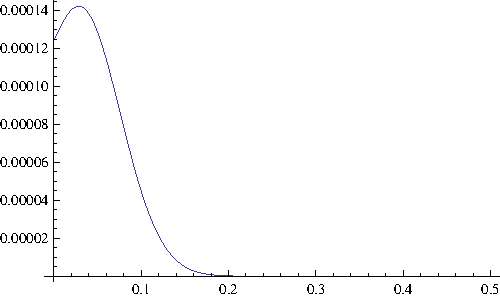
\includegraphics[width=.9\textwidth]{myp}
\caption{The function $P(x)$ shown over the domain from $x_0 = 0.5 $ to the branching point, 0.}
\end{center}
\end{figure}

\begin{figure}
\begin{center}
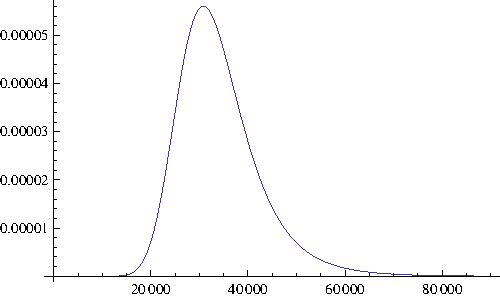
\includegraphics[width=.9\textwidth]{mywaiting}
\caption{The distribution of waiting times from this approximation.  This distribution has a mean of 34130, and variance $4.4\cdot 10^7$.}
\end{center}
\end{figure}

\begin{figure}
\begin{center}
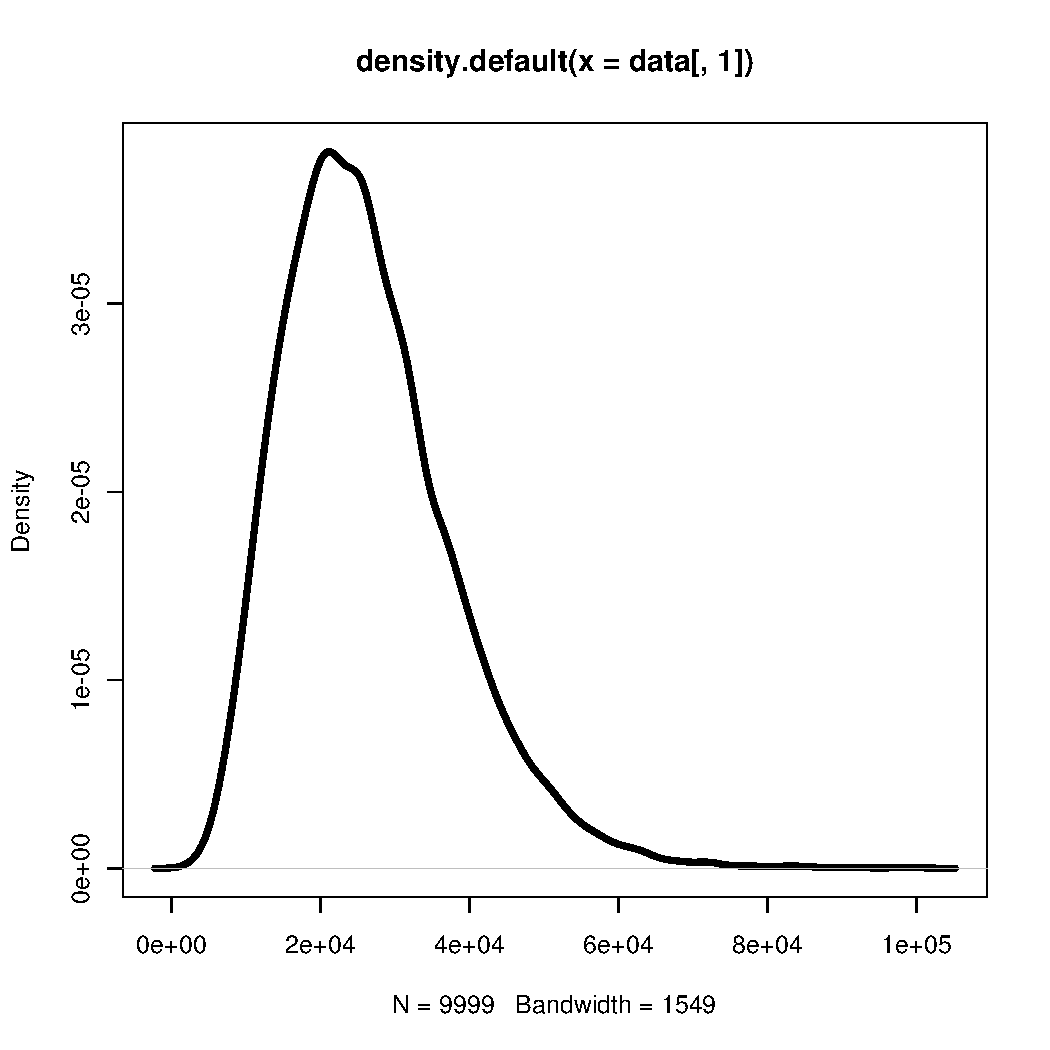
\includegraphics[width=.9\textwidth]{waittimes}
\caption{The distribution of waiting times from the simulation (smoothing by kernel density estimation).   This distribution has a mean of 26330, and variance $12.9\cdot 10^7$.}
\end{center}
\end{figure}




\subsection{Coexistence}
Consider a population of two coexisting types, characterized by traits $x_1$ and $x_2$ respectively.  The birth and death rates of each population are then given by expression ~\eqref{general_logistic}.  We'll assume that the populations can coexist, that is $(x_1, x_2)$ falls into the coexistence region $P_2$; \emph{i.e.} that $C(x_1,x_2)K(x_2) /K_1(x_1) < 1 $ and $C(x_1, x_2) K(x_1)/K(x_2) < 1$.  This guarentees that each population has a positive expected growth rate when rare.  However, because the population is composed of finitely many discrete individuals, there is still a chance that either type will be lost to chance; to demographic stochasticity.  We whish to characterize the expected waiting time for such an event to occur. 

To do so, we will switch first into density and then frequency, to obtain a one-dimensional expression we can solve exactly.  We will then use the Arhennius approximation to obtain a closed form solution.  First, we will replace the discrete number of individuals $N$ with the macroscopic, continuous variable $n$, representing the mean \emph{density} of individuals; $N/A$, where $A$ is the area in which $N$ individuals are found.  For suitably large $A$, we will be able to accurately describe $n$ with a coupled stochastic differential equation for each population.  By changing variables once more into the frequency of one type, $p = n_1/(n_1+n_2)$ and $n = n_1 + n_2$, we are able to do a timescale seperation to focus on the dynamics in a single variable, $p$.  


The master equation that describes the probability of observing $N_i$ individuals of type $i$ is given by,

\begin{align}
\frac{\ud}{\ud t} P(N_1,t) &= (\E_1 - 1) r N_1 \frac{N_1 + C(x_1, x_2) N_2}{K(x_1) }P(N_1) + (\E_1^{-1} - 1)r N_1 P(N_1) \nonumber \\
\frac{\ud}{\ud t} P(N_2,t) &= (\E_2 - 1) r N_2 \frac{N_2 + C(x_2, x_1) N_1}{K(x_2) }P(N_2) + (\E_2^{-1} - 1)r N_2 P(N_2)
\label{mastereq}
\end{align}
where $\E_i^k$ is the step operator taking $f(N_i) \to f(N_{i+k})$.  We apply van Kampen's expansion of the master equation to linear order to recover the following stochastic differential equation (It\^o equation)

\begin{align}
\ud n_1 = r n_1 \left(1 -  \frac{n_1 + C(x_1, x_2) n_2}{K(x_1) } \right) \ud t + \frac{1}{\sqrt{K_o} } \sqrt{r n_1 \left(1 +  \frac{n_1 + C(x_1, x_2) n_2}{K(x_1) } \right) } \ud W_1
\label{sde}
\end{align}
and $n_2$ similarly.  Switching into the variables for frequency, $p = n_1/n$ and $n = n_1+n_2$ and simplying notation by $C(x_1, x_2) = c_{12}$ and $K(X_i) = k_i$:

\begin{align}
\ud p &= r p \left(1 -  n(p) \frac{p + c_{12}(1-p) }{k_1 } \right) \ud t + \frac{1}{\sqrt{K_o n(p)} } \sqrt{r p \left(1 +  n(p)\frac{p + c_{12} (1-p) }{k_1 } \right) } \ud W_1  \label{freq_sde} \\
n(p) &=  \frac{k_1 k_2}{k_2 p^2 + (k_1+k_2) c_{12} p (1-p) + k1 (1-p)^2 }, 
\end{align}

where we have set the dynamic equation for $n(p)$ to equilibrium.  The extinction probability $u(p,t)$ for this expression is given by the Backwards equation for the generator,
\begin{equation}
\frac{\ud}{\ud t} u(p,t) = \underbrace{r p \left(1 -  n(p) \frac{p + c_{12}(1-p) }{k_1 } \right)}_{A(p)} \partial_p u(p,t) + \tfrac{1}{2} \underbrace{\frac{1}{K_o n(p) } r p \left(1 +  n(p)\frac{p + c_{12} (1-p) }{k_1 } \right)}_{B(p)} \partial_p^2 u(p,t) 
\label{u}
\end{equation}
with the boundary conditions $u(0,t) = 1$ and $u(1,t) = 1$ being absorbing.  



Assuming that type 1 is the rare mutant invader, we can solve this explicitly for small $p$, and particularly for the case of exactly one new mutant.  After some rearrangement we can rewrite this as 
\begin{multline}
\frac{\ud}{\ud t} u(p,t) = \left( rp \left( 1-\frac{n c_{12}}{k_1} \right) - \frac{r n}{k_1} p^2 (1 - c_{12} )\right)  \partial_p u(p,t) \\
+ \left( rp \left(1+\frac{n c_{12}}{k_1}\right)  + \frac{r n }{k_1} p^2 (1 - c_{12} ) \right) \frac{\partial_p^2 u(p,t)}{2K_0 n}
\end{multline}
Note then for $p$ small we can neglect the terms quadratic in $p$ and we are left with the backwards equation from the density independent case, 
\begin{equation}
\frac{\ud}{\ud t} u(p,t) =  rp \left( 1-\frac{n c_{12}}{k_1} \right)   \partial_p u(p,t) + rp \left(1+\frac{n c_{12}}{k_1}\right)   \frac{\partial_p^2 u(p,t)}{2K_0 n}
\end{equation}
Setting equal to zero we have a simple ordinary differential equation for the stationary extinction probability:
\begin{align}
u(p) &= 1 - e^{-2sp K_0 n} \\
s &= \frac{r\left( 1-\frac{n c_{12}}{k_1} \right) }{ r\left(1+\frac{n c_{12}}{k_1}\right)} 
\end{align}
and particularly for a frequency $p$ corresponding to a single individual, a frequency of $p=1/(N_1+N_2) =(1/K_0)/(n_1+n_2) = 1/(K_0 n)$, this reduces to
\begin{equation}
u = 1-e^{-2s}
\end{equation}
Assuming $ rp \left( 1-\frac{k_2 c_{12}}{k_1} \right) \neq 0$, the time-dependent solution\footnote{note that $n(p) \approx k_2$ for small $p$.} is:
\begin{align}
u(p,t) &= 1-e^{-p \psi(t) } \\
\psi(t) &= \frac{2 s K_0 n}{1-e^{ r\left( 1-\frac{k_2 c_{12}}{k_1} \right) t } }
\label{timedep}
\end{align}

Larger population (system size) $K_o$ results in longer persistance.  

This tells us nothing about the survival of the resident, as it is only valid for small $p$.  In most applications of this approach, it is assumed the resident quickly goes extinct once $p \sim o(1)$.  If we consider the asymptotic behavior of the nonlinear PDE, Eq.~\eqref{u}, we see sure absorbtion at one boundary or the other. The asymptotic behavior needn't concern us; as we really want to know how the expected lifetime of this dimporphic state compares with the rate at which mutants are entering this population. To do so we need the time dependent solution to the nonlinear backwards equation~\eqref{u}.    

While a direct solution to the nonlinear PDE is not available, we can solve for the moments analytically.  As $u(p,t)$ is the probability of non-extinction, that is, that the exit time $T$ is greater than the current time $t$; e.g. $u$ is the cumululative probability density.  Consequently the mean exit time $T(p)$ is given by,

\begin{equation}
T(p) = - \int_0^\infty t \partial_t u(p,t) \ud t = \int_0^\infty u(p,t) \ud t \label{simple} 
\end{equation}

where we have integrated by parts to get the second expression.  Meanwhile, we can integrate the left-hand side of~\eqref{u}, 
\begin{equation*}
\int_0^{\infty} \partial_t u(p,t) \ud t = u(p,\infty) - u(p,0) = -1
\end{equation*}
and integrate the right hand side using~\eqref{simple} to get
\begin{equation*}
A(p) \partial_p T(p) + \tfrac{1}{2} B(p) \partial_p^2 T(x) = -1
\end{equation*}

This can be integrated directly to solve for the mean time starting from $p=x$ to be absorbed at either boundary $a=0$ or $b=1$:

\begin{align}
T(x) &= \frac{2 \left[\left(\int_a^x\frac{\ud y}{\psi(y)}\right)\int_x^b \frac{\ud y'}{\psi(y')} \int_a^{y'} \frac{\ud z \psi(z)}{B(z)} - \left(\int_x^b\frac{\ud y}{\psi(y)}\right)\int_a^x \frac{\ud y'}{\psi(y')} \int_a^{y'} \frac{\ud z \psi(z)}{B(z)}\right]}{\int_a^b \frac{\ud y}{\psi(y)}}
\label{7integrals} 
\intertext{where}
\psi(x) &= \exp\left( \int_0^x \ud x' \frac{2A(x')}{B(x')} \right)
\end{align}

Though these integrals can be computed numerically, a small noise limit (large populations) allows us to make an additional approximation by mapping this problem onto the familiar question of escape over a potential energy barrier.  This question arises in basic chemistry, and is described by a similar stochastic differential equation where the $A(x)$ coefficent represents the gradient of the energy surface and $B$ the temperature.  The analogy initially appears to fail, since in the chemical context the diffusion coefficent is determined by the temperature alone, and is independent of the state, while our $B$ term depends on the frequency $p$.  However, as it is not explicitly time dependent, there is always a transform to change variables into a context where $B$ is constant.  The relevant transformation for us is known as the Lamperti Transform.  Switching variables from $p$ to $q$ by means of the transform:

\begin{equation}
q = F(p) = \int_z^{p} \frac{1}{\sqrt{B(u)}} \ud u
\label{p_to_q}
\end{equation}

we can rewrite~\eqref{u} as

\begin{align}
\frac{\partial u(q,t)}{\partial t} = \underbrace{\left(\frac{4 A(p)- \partial_p B(p) }{4\sqrt{B(p)}}  \right)}_{\nabla V(p)} \frac{\partial u(q,t)}{\partial q} + \frac{1}{2} \frac{\partial^2 u(q,t)}{\partial q^2}.
\label{new_u}
\end{align}

The mean first passage time in this transformed variable is still solved by~\eqref{7integrals}.  However, interpreting the coefficent of the drift term as the gradient of the energy landscape, $\nabla V(p)$, we can approximate that this time will scale as the exponent of the depth of the energy well defined by that landscape:

\begin{equation}
\exp{- (\min(V(0), V(1)) - V(p^*) )}
\end{equation}




\section{Results}
\begin{figure}
\begin{center}
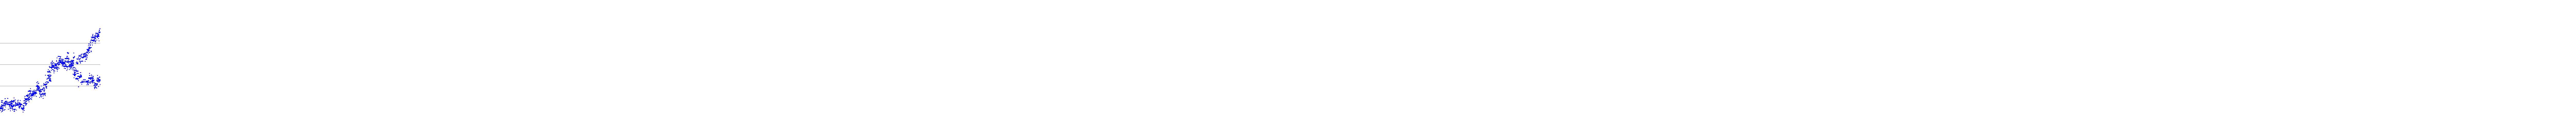
\includegraphics[height= 4cm, width=\textwidth]{short.jpg}

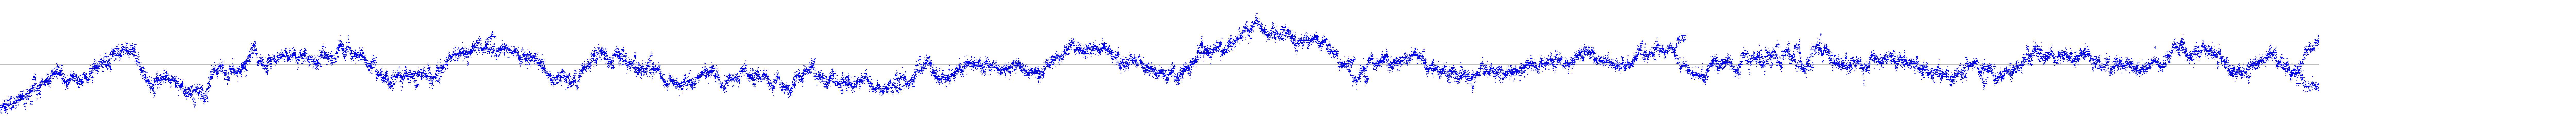
\includegraphics[height=4cm, width=\textwidth]{long.jpg}
\end{center}
\caption{$N = 100, MK = 0.50, MC= 3 \sigma_{\mu} = 3.0e-02, \mu = 1.0e-02$}
\label{fig:times}
\end{figure}

\bibliography{mycanonical.bib}

\end{document}


Suppose we have the stochastic differential equation:

\begin{equation}
\ud X_t = A(t,X_t)\ud t + \sqrt{B(X_t)} \ud W_t
\label{general_sde}
\end{equation}

We apply the Lamperti transform,

\begin{equation}
Y_t = F(X_t) = \int_z^{X_t} \frac{1}{\sqrt{B(u)}} \ud u
\label{lamperti}
\end{equation}

where the process $Y_t$ solves the stochastic differential equation

\begin{align}
\ud Y_t = \left(\frac{A(t,X_t)}{\sqrt{B(X_t)}} - \frac{\partial_{X_t} B(X_t) }{4 \sqrt{B(X_t)} } \right) \ud t + \ud W_t.
\label{transformed}
\end{align}




